\section{Dataset Normalization}
%% How to represent input tensor, to make it fast converse

The vertices have been normalized before feed them into the model. The depth range of each scene is shown in Figure \ref{fig:data_range}.
The sizes of each training object are various, whereas it should be as an invariant value for the training model. Thus the normalization is required before feed training objects into the models. Figure \ref{fig:data_range} shows the fluctuation of extreme values and their ranges in 100 random training items. Table \ref{tab:data_range} gives the corresponding average values.
%\begin{figure}[!h]
%	\centering
%	{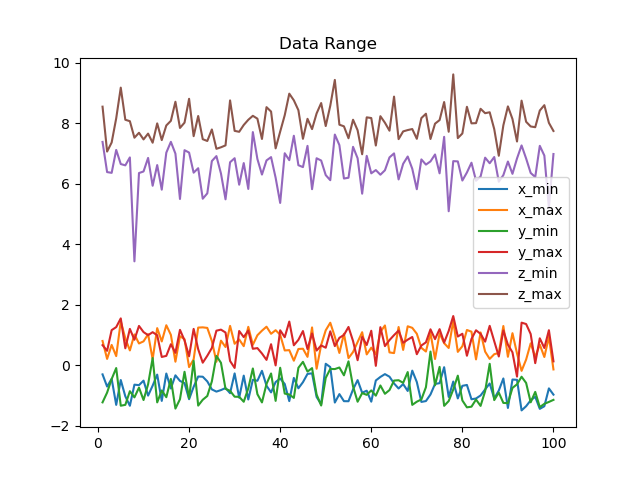
\includegraphics[width=0.45\textwidth]{./pic/Data_Extreme.png}}
%	{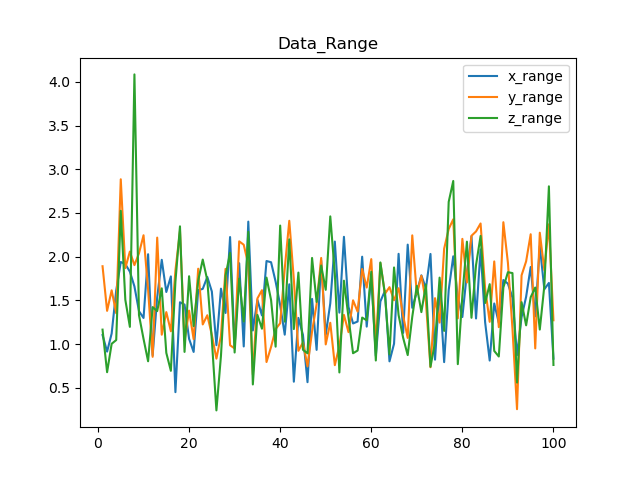
\includegraphics[width=0.45\textwidth]{./pic/Data_Range.png}}
%	\label{fig:data_range}
%	\caption{Left: Extreme value in 3 axis; Right: Vertex range in 3 axis}
%\end{figure}

\begin{table}[!h]
	\centering
	\begin{tabular}{|c|c|c|c|}
		\hline
		Axis & Range & Min & Max\\
		\hline
		X & 1.48 & -0.75 & 0.73\\
		Y & 1.56 & -0.76 & 0.80\\
		Z & 1.47 & 6.53 & 8.00\\
		\hline
	\end{tabular}
	\caption{The ranges and extreme values of each axis. The extreme min and max values of both X axis and Y axis are close to $ -0.75 $ and $ 0.75 $ separately. The case for Z axis is $ 6.5 $ and $ 8.0 $ separately. However, the range of three axes are relatively similar, around 1.5. 
	}
	\label{tab:data_range}
\end{table}


For the normalization, first we translate the point to the original point as much as possible, then choose the range value of one axis as a scale factor, normalize it to a unit object. 

\begin{equation}\label{eq:normalization}
	U^a = (V^a - V^a_{min}) / s  \quad  \text{for } a \text{ in }  X,Y,Z \text{ axis}
\end{equation}
where $ V^a_{min} $ denote the minimum value appeared in axis $ a $, $ s $ is the range of an axis, which can be any one of X, Y, or Z axis.
